\documentclass[a4paper]{article}
\usepackage{vntex}
\usepackage{a4wide,amssymb,epsfig,latexsym,array,hhline,fancyhdr}
\usepackage{amsmath}
\usepackage{amsthm}
\usepackage{multicol,longtable,amscd}
\usepackage{diagbox}
\usepackage{booktabs}
\usepackage{alltt}
\usepackage[framemethod=tikz]{mdframed}
\usepackage{caption,subcaption}
\usepackage{lastpage}
\usepackage[lined,boxed,commentsnumbered]{algorithm2e}
\usepackage{enumerate}
\usepackage{color}
\usepackage{graphicx}
\usepackage{array}
\usepackage{tabularx, caption}
\usepackage{multirow}
\usepackage{multicol}
\usepackage{rotating}
\usepackage{graphics}
\usepackage{geometry}
\usepackage{setspace}
\usepackage{epsfig}
\usepackage{tikz}
\usepackage[british]{babel}

\usetikzlibrary{arrows,snakes,backgrounds}
\usepackage[unicode]{hyperref}
\hypersetup{urlcolor=blue,linkcolor=black,citecolor=black,colorlinks=true}

\setlength{\headheight}{40pt}
\pagestyle{fancy}
\fancyhead{} % clear all header fields
\fancyhead[L]{
 \begin{tabular}{rl}
    \begin{picture}(25,15)(0,0)
    \put(0,-8){
\includegraphics[width=8mm, height=8mm]{image/local/hcmut.png}}
    %\put(0,-8){\epsfig{width=10mm,figure=hcmut.eps}}
   \end{picture}&
	%
\includegraphics[width=8mm, height=8mm]{hcmut.png} & %
	\begin{tabular}{l}
		\textbf{\bf \ttfamily Trường Đại Học Bách Khoa Tp.Hồ Chí Minh}\\
		\textbf{\bf \ttfamily Khoa Khoa Học và Kỹ Thuật Máy Tính}
	\end{tabular}
 \end{tabular}
}
\fancyhead[R]{
	\begin{tabular}{l}
		\tiny \bf \\
		\tiny \bf
	\end{tabular}  }
\fancyfoot{} % clear all footer fields
\fancyfoot[L]{\scriptsize \ttfamily GIAI ĐOẠN 1: ĐỀ CƯƠNG LUẬN VĂN/ ĐỒ ÁN CHUYÊN NGÀNH/
ĐỒ ÁN MÔN HỌC KỸ THUẬT MÁY TÍNH - HỌC KỲ 2 NĂM HỌC 2023-2024}
\fancyfoot[R]{\scriptsize \ttfamily Trang {\thepage}/\pageref{LastPage}}
\renewcommand{\headrulewidth}{0.3pt}
\renewcommand{\footrulewidth}{0.3pt}

\setcounter{secnumdepth}{4}
\setcounter{tocdepth}{3}
\makeatletter
\newcounter {subsubsubsection}[subsubsection]
\renewcommand\thesubsubsubsection{\thesubsubsection .\@alph\c@subsubsubsection}
\newcommand\subsubsubsection{\@startsection{subsubsubsection}{4}{\z@}%
                                     {-3.25ex\@plus -1ex \@minus -.2ex}%
                                     {1.5ex \@plus .2ex}%
                                     {\normalfont\normalsize\bfseries}}
\newcommand*\l@subsubsubsection{\@dottedtocline{3}{10.0em}{4.1em}}
\newcommand*{\subsubsubsectionmark}[1]{}
\makeatother

\sloppy
\captionsetup[figure]{labelfont={small,bf},textfont={small,it},belowskip=0pt,aboveskip=0pt}
\captionsetup[table]{labelfont={small,bf},textfont={small,it},belowskip=-1pt,aboveskip=7pt}
\setlength{\floatsep}{5pt plus 2pt minus 2pt}
\setlength{\textfloatsep}{5pt plus 2pt minus 2pt}
\setlength{\intextsep}{10pt plus 2pt minus 2pt}

\begin{document}

\begin{titlepage}
\begin{center}
ĐẠI HỌC QUỐC GIA THÀNH PHỐ HỒ CHÍ MINH \\
TRƯỜNG ĐẠI HỌC BÁCH KHOA \\
KHOA KHOA HỌC - KỸ THUẬT MÁY TÍNH
\end{center}

\vspace{1cm}

\begin{figure}[h!]
\begin{center}

\includegraphics[width=4cm]{image/local/hcmut.png}
\end{center}
\end{figure}
\vspace{1cm}
\begin{center}
\begin{tabular}{c}
\multicolumn{1}{l}{\textbf{{\Large GIAI ĐOẠN 1 (GĐ1):}}}\\
\multicolumn{1}{l}{\textbf{{ĐỀ CƯƠNG LUẬN VĂN/ ĐỒ ÁN CHUYÊN NGÀNH/}}}\\
\multicolumn{1}{l}{\textbf{{ĐỒ ÁN MÔN HỌC KỸ THUẬT MÁY TÍNH}}}\\
~~\\
\hline
\\
\multicolumn{1}{l}{\textbf{{\Large Tên đề tài}}}\\
\multicolumn{1}{l}{\textbf{{Tiếng Việt: Rút trích quan hệ giữa Ý định và Thực thể}}}\\
\multicolumn{1}{l}{\textbf{{ sử dụng hướng tiếp cận Đọc hiểu Máy}}}\\
\multicolumn{1}{l}{\textbf{{ cho nhiệm vụ xây dựng Đồ thị Tri thức trong lĩnh vực Giáo dục.}}}\\
\\
\multicolumn{1}{l}{\textbf{{Tiếng Anh: Relation Extraction between}}}\\
\multicolumn{1}{l}{\textbf{{ Intent and Entity using Machine Reading Comprehension(MRC)}}}\\
\multicolumn{1}{l}{\textbf{{ approach for Knowledge}}}\\
\multicolumn{1}{l}{\textbf{{ Graph Construction in Education domain.}}}\\


\\
\hline
\end{tabular}
\end{center}

\vspace{0.7cm}

\begin{table}[h]
\centering \large
\begin{tabular}{rll}
\textbf{Giáo viên hướng dẫn:} & Bùi Công Tuấn &   \\
 & & \\
\textbf{SV thực hiện:} & Lưu Quốc Bình & 2033009  \\

\end{tabular}
\end{table}

\vspace{1.0cm}
\begin{center}
{\footnotesize Tp. Hồ Chí Minh, Tháng 05 Năm 2024}
\end{center}
\end{titlepage}

\newpage
\tableofcontents
\newpage

%%%%%%%%%%%%%%%%%%%%%%%%%%%%%%%%%%%%%%%%%%%%%%%%%%%%%%%%%%%%%%%%%%%


\newpage
\section{Database Integration}
\subsection{Bottom-Up Design Methodology}
Thiết kế Bottom-up \\

Có hai cách tiếp cận
\begin{itemize}
    \item
    \item GCS được coi như là phẩn liên kết của LCS
\end{itemize}

\subsection{Schema Matching}

\begin{figure}
    \centering
    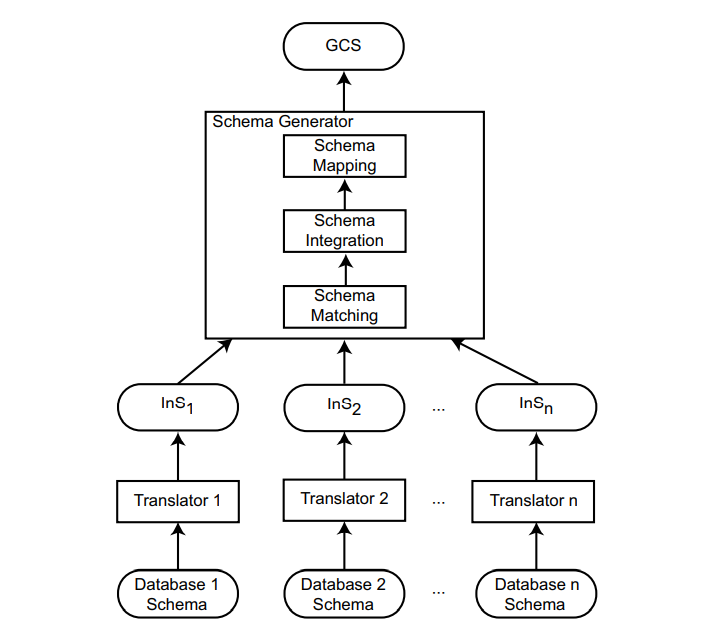
\includegraphics[]{image/chap4/DBIntegrationProc.PNG}
    \caption{Database Integration Process}
\end{figure}



\subsection{Schema Integration}
\subsection{Schema Mapping}
Sau khi GCS (global conceptual schema) được xác định, cần phải thiết kế cách để dữ liệu từ từng cơ sở dữ liệu cục bộ (từ nguồn) có thể ánh xạ lên GCS (đích) cần dùng mà vẫn duy trì tính nhất quán về ngữ nghĩa (như được xác định bởi từ nguồn và đích). Mặc dù ánh xạ lược đồ đã xác định được sự tương ứng giữa các LCS và GCS, nó vẫn chưa thể xác định rõ ràng cách lấy cơ sở dữ liệu toàn cục từ các cơ sở dữ liệu cục bộ. Đây là những gì ánh xạ lược đồ nói về

\subsection{Data Cleaning}
Các lỗi trong cơ sở dữ liệu nguồn luôn có thể xảy ra, yêu cầu phải làm sạch để làm chính xác
trả lời các truy vấn của người dùng. Làm sạch dữ liệu là một vấn đề nảy sinh trong cả hai kho dữ liệu
và các hệ thống tích hợp dữ liệu, nhưng trong các bối cảnh khác nhau. Trong kho dữ liệu, nơi
dữ liệu thực sự được trích xuất từ cơ sở dữ liệu hoạt động cục bộ và được vật chất hóa dưới dạng
cơ sở dữ liệu toàn cầu, việc dọn dẹp được thực hiện khi cơ sở dữ liệu toàn cầu được tạo. Trong trường hợp
của hệ thống tích hợp dữ liệu, làm sạch dữ liệu là một quá trình cần được thực hiện
trong quá trình xử lý truy vấn khi dữ liệu được trả về từ cơ sở dữ liệu nguồn.

Các lỗi trong source database luôn có thể xảy ra, yêu cầu phải làm sạch để xác định chính xác
trả lời các câu hỏi của người dùng. Làm sạch dữ liệu là một vấn đề nảy sinh trong cả hai kho dữ liệu
và dữ liệu tích hợp hệ thống, but trong các bối cảnh khác nhau. Trong kho dữ liệu, seek
thực tế dữ liệu được trích xuất từ cục bộ cơ sở dữ liệu và được vật chất hóa dưới dạng
toàn bộ cơ sở dữ liệu, công việc dọn dẹp được thực hiện khi cơ sở dữ liệu được yêu cầu được tạo ra. Trong trường hợp của hệ thống dữ liệu, thực hiện dữ liệu sạch là một quá trình được thực hiện trong quá trình truy vấn khi dữ liệu được trả về từ cơ sở dữ liệu nguồn.


Cách tiếp cận phổ biến để làm sạch dữ liệu là xác định một số toán tử
hoạt động trên lược đồ hoặc trên dữ liệu riêng lẻ. Các toán tử có thể được bao gồm
vào một kế hoạch làm sạch dữ liệu. Các toán tử giản đồ mẫu thêm hoặc bớt các cột từ bảng,
cấu trúc lại bảng bằng cách kết hợp các cột hoặc tách một cột thành hai [Raman
và Hellerstein, 2001], hoặc xác định phép biến đổi giản đồ phức tạp hơn thông qua
toán tử "bản đồ" chung [Galhardas và cộng sự, 2001] nhận một quan hệ duy nhất và
tạo ra một quặng nhiều quan hệ hơn. Các toán tử cấp dữ liệu mẫu bao gồm những toán tử
áp dụng một hàm cho mọi giá trị của một thuộc tính, hợp nhất các giá trị của hai thuộc tính thành
giá trị của một thuộc tính đơn lẻ và toán tử phân tách ngược của nó [Raman và Hellerstein,
2001], một toán tử so khớp tính toán một phép nối gần đúng giữa các bộ giá trị
hai quan hệ, toán tử phân cụm nhóm các bộ giá trị của một quan hệ thành các cụm và một
toán tử hợp nhất tuple phân chia các bộ giá trị của một quan hệ thành các nhóm và thu gọn
các bộ trong mỗi nhóm thành một bộ duy nhất thông qua một số tập hợp trên chúng
[Galhardas và cộng sự, 2001], cũng như các toán tử cơ bản để tìm các bản sao và loại bỏ
chúng (đây từ lâu đã được gọi là vấn đề thanh trừng / hợp nhất [Hernandez và Stolfo, ´
1998]). Nhiều toán tử mức dữ liệu so sánh các bộ giá trị riêng lẻ của hai quan hệ
(từ các lược đồ giống nhau hoặc khác nhau) và quyết định xem chúng có đại diện cho
cùng một thực tế. Điều này tương tự như những gì được thực hiện trong đối sánh giản đồ, ngoại trừ việc nó được thực hiện
ở cấp dữ liệu riêng lẻ và những gì được coi là không phải là các giá trị thuộc tính riêng lẻ,
nhưng toàn bộ bộ giá trị. Tuy nhiên, các kỹ thuật tương tự mà chúng tôi đã nghiên cứu trong đối sánh lược đồ
(ví dụ: sử dụng khoảng cách chỉnh sửa hoặc giá trị soundex) có thể được sử dụng trong ngữ cảnh này. Ở đây có
là đề xuất cho các kỹ thuật đặc biệt để xử lý điều này một cách hiệu quả trong bối cảnh
làm sạch dữ liệu (ví dụ, [Chaudhuri và cộng sự, 2003]).

Với lượng lớn dữ liệu cần được xử lý, việc làm sạch mức dữ liệu là
đắt tiền và hiệu quả là một vấn đề quan trọng. Việc thực hiện vật lý của mỗi
của các toán tử mà chúng ta đã thảo luận ở trên là một mối quan tâm đáng kể. Mặc dù vệ sinh có thể
được thực hiện ngoại tuyến như một quy trình hàng loạt trong trường hợp kho dữ liệu, để tích hợp dữ liệu
hệ thống, việc làm sạch cần được thực hiện trực tuyến vì dữ liệu được truy xuất từ ​​các nguồn. Các
tất nhiên, hiệu suất làm sạch dữ liệu quan trọng hơn trong trường hợp thứ hai. Trên thực tế
mối quan tâm về hiệu suất và khả năng mở rộng trong các hệ thống sau này đã dẫn đến các đề xuất
trong đó việc làm sạch dữ liệu bị hủy bỏ để có lợi cho truy vấn có thể chấp nhận được xung đột [Yan
và Ozsu, 1999] ¨.

\subsection{Kết luận}
Trong phần này, chúng mình đã thảo luận về quy trình thiết kế cơ sở dữ liệu từ dưới lên,có tên gọi là
tích hợp cơ sở dữ liệu (Database Integration). Đây là quá trình tạo GCS (global conceptual schema)
và xác định cách mỗi LCS (local conceptual schema) ánh xạ tới nó. Một sự tách biệt cơ bản là giữa
kho dữ liệu nơi GCS được khởi tạo và hiện thực hóa cũng như tích hợp dữ liệu
hệ thống mà GCS chỉ là một chế độ xem ảo.

Mặc dù chủ đề tích hợp cơ sở dữ liệu đã được nghiên cứu nhiều cho một
lâu nay hầu như toàn bộ công việc bị rời rạc. Các dự án cá nhân tập trung vào
đối sánh giản đồ, hoặc làm sạch dữ liệu, hoặc ánh xạ lược đồ. Thiếu nghiêm trọng
nghiên cứu xem xét phương pháp luận end-to-end để tích hợp cơ sở dữ liệu. Sự thiếu
một phương pháp luận được thực hiện nghiêm túc hơn bởi thực tế là mỗi hoạt động nghiên cứu này
làm việc trên các giả định khác nhau liên quan đến mô hình dữ liệu, các loại không đồng nhất, v.v.
trên. Một ngoại lệ đáng chú ý là công trình của Bernstein và Melnik [2007], cung cấp
sự khởi đầu của một phương pháp luận toàn diện “từ đầu đến cuối”. Đây có lẽ là
chủ đề quan trọng nhất cần được chú ý.

Một khái niệm liên quan đã được thảo luận đáng kể trong tài liệu là dữ liệu
đổi. Đây được định nghĩa là “vấn đề lấy dữ liệu có cấu trúc theo một nguồn
lược đồ và tạo một phiên bản của lược đồ mục tiêu phản ánh dữ liệu nguồn
Càng chính xác càng tốt." [Fagin và cộng sự, 2005]. Điều này rất giống với vật lý
tích hợp dữ liệu tích hợp (tức là hiện thực hóa), chẳng hạn như kho dữ liệu, mà chúng tôi
được thảo luận trong chương này. Sự khác biệt giữa kho dữ liệu và các phương pháp tiếp cận materializa tion như được đề cập trong môi trường trao đổi dữ liệu là kho dữ liệu
dữ liệu thường thuộc về một tổ chức và có thể được cấu trúc theo một lược đồ được xác định rõ ràng trong khi trong môi trường trao đổi dữ liệu, dữ liệu có thể đến từ các
nguồn và chứa không đồng nhất [Doan et al., 2010]. Tuy nhiên, đối với hầu hết các
thảo luận của chương này, đây không phải là một mối quan tâm lớn.

Trọng tâm của chúng tôi trong chương này là tích hợp cơ sở dữ liệu. Tuy nhiên, càng ngày,
dữ liệu được sử dụng trong các ứng dụng phân tán liên quan đến những dữ liệu không có trong
cơ sở dữ liệu. Một chủ đề thảo luận mới thú vị giữa các nhà nghiên cứu là sự tích hợp
dữ liệu có cấu trúc được lưu trữ trong cơ sở dữ liệu và dữ liệu phi cấu trúc được duy trì
trong các hệ thống khác (máy chủ Web, hệ thống đa phương tiện, thư viện kỹ thuật số, v.v.) [Halevy
và cộng sự, 2003; Somani và cộng sự, 2002]. Trong các hệ thống thế hệ tiếp theo, khả năng xử lý cả hai
các loại dữ liệu sẽ ngày càng quan trọng.

Một vấn đề khác mà chúng tôi đã bỏ qua trong chương này là khả năng tương tác khi GCS
không tồn tại hoặc không thể được chỉ định. Như chúng ta đã thảo luận trong Chương 1, đã sớm có
phản đối quyền truy cập tương thích vào nhiều nguồn dữ liệu thông qua GCS, tranh luận
thay vào đó, các ngôn ngữ phải cung cấp các phương tiện để truy cập vào nhiều
nguồn mà không yêu cầu GCS. Vấn đề trở nên quan trọng trong các hệ thống ngang hàng hiện đại, nơi mà quy mô và sự đa dạng của các nguồn dữ liệu gây ra khá nhiều khó khăn
(nếu không phải là không thể) để thiết kế một GCS. Chúng ta sẽ thảo luận về tích hợp dữ liệu trong peer-to-peer
hệ thống trong Chương 16.

\newpage

\section{Multidatabase Query Processing}
\subsection{Issues in Multidatabase Query Processing}
Xử lý truy vấn trong hệ thống đa cơ sở dữ liệu phức tạp hơn trong hệ thống phân tán DBMS vì những lý do sau:
\begin{itemize}
    \item Khả năng tính toán của các DBMS thành phần có thể khác nhau, ngăn việc xử lý đồng nhất các truy vấn trên nhiều DBMS. Ví dụ, một số DBMS có thể hỗ trợ các truy vấn SQL phức tạp với phép nối và tổng hợp trong khi một số khác không thể. Do đó, bộ xử lý truy vấn đa cơ sở dữ liệu nên xem xét các khả năng DBMS khác nhau.
    \item Tương tự, chi phí xử lý các truy vấn có thể khác nhau trên các DBMS khác nhau, và khả năng tối ưu hóa cục bộ của mỗi DBMS có thể khác nhau. Điều này làm tăng độ phức tạp của các hàm chi phí cần được đánh giá.
    \item Các mô hình dữ liệu và ngôn ngữ của các DBMS thành phần có thể khá khác nhau, ví dụ, quan hệ, hướng đối tượng, XML, v.v. Điều này tạo ra khó khăn trong việc dịch các truy vấn đa cơ sở dữ liệu sang DBMS thành phần và trong tích hợp các kết quả không đồng nhất.
    \item Vì hệ thống đa cơ sở dữ liệu cho phép truy cập vào các DBMS rất khác nhau có thể có hiệu suấ và hành vi khác nhau, xử lý truy vấn phân tán các kỹ thuật cần phải thích ứng với những biến thể này.
\end{itemize}
Quyền tự chủ của các DBMS thành phần đặt ra nhiều vấn đề. Quyền tự chủ của DBMS có thể được định nghĩa theo ba khía cạnh chính: giao tiếp, thiết kế và thực thi [Lu et al., 1993]. Quyền tự chủ về giao tiếp có nghĩa là một DBMS thành phần giao tiếp với những người khác theo quyết định riêng của nó, và đặc biệt, nó có thể chấm dứt các dịch vụ của mình bất kỳ lúc nào. Điều này đòi hỏi các kỹ thuật xử lý truy vấn chịu được sự không khả dụng của hệ thống. Câu hỏi đặt ra là làm thế nào hệ thống trả lời các truy vấn khi một hệ thống thành phần không khả dụng ngay từ đầu hoặc tắt khi đang thực thi truy vấn. Quyền tự chủ về thiết kế có thể hạn chế tính khả dụng và độ chính xác của thông tin chi phí cần thiết để tối ưu hóa truy vấn. Khó khăn trong việc xác định các hàm chi phí địa phương là một vấn đề quan trọng. Quyền tự chủ thực thi của các hệ thống đa cơ sở dữ liệu gây khó khăn cho việc áp dụng một số chiến lược tối ưu hóa truy vấn mà chúng ta đã thảo luận trong các chương trước. Ví dụ: tối ưu hóa dựa trên bán liên kết của các phép nối phân tán có thể khó khăn nếu quan hệ nguồn và đích nằm trong các DBMS thành phần khác nhau, vì, trong trường hợp này, việc thực thi bán liên kết của một phép nối chuyển thành ba truy vấn: một truy vấn để truy xuất các giá trị thuộc tính nối của quan hệ đích và chuyển nó đến DBMS của quan hệ nguồn, thứ hai để thực hiện phép nối tại mối quan hệ nguồn và mối quan hệ thứ ba để thực hiện phép nối tại DBMS của quan hệ đích. Vấn đề nảy sinh do giao tiếp với các DBMS thành phần xảy ra ở cấp cao của API DBMS.


Ngoài những khó khăn này, kiến trúc của một cơ sở dữ liệu đa cơ sở phân tán
hệ thống đặt ra những thách thức nhất định. Kiến trúc được mô tả trong Hình 1.17 trỏ đến một
phức tạp bổ sung. Trong các DBMS phân tán, bộ xử lý truy vấn chỉ phải xử lý
phân phối dữ liệu trên nhiều trang web. Trong môi trường đa cơ sở dữ liệu phân tán,
mặt khác, dữ liệu không chỉ được phân phối trên các trang web mà còn trên nhiều cơ sở dữ liệu, mỗi cơ sở dữ liệu được quản lý bởi một DBMS tự trị. Như vậy, trong khi có hai bên
hợp tác trong việc xử lý các truy vấn trong một DBMS phân tán (trang web kiểm soát
và các trang web địa phương), số lượng các bên tăng lên ba trong trường hợp
đa DBMS: lớp đa DBMS tại vị trí điều khiển (tức là người trung gian) nhận được
truy vấn toàn cục, các lớp đa DBMS tại các trang web (tức là các trình bao bọc) tham gia
trong quá trình xử lý truy vấn và các DBMS thành phần cuối cùng tối ưu hóa và thực thi
truy vấn.

\subsection{Multidatabase Query Processing Architecture}
Hầu hết công việc xử lý truy vấn đa cơ sở dữ liệu đã được thực hiện trong ngữ cảnh
của kiến trúc trình trung gian / trình bao bọc (xem Hình 1.18). Trong kiến trúc này, mỗi
cơ sở dữ liệu thành phần có một trình bao bọc được liên kết xuất thông tin về
lược đồ nguồn, dữ liệu và khả năng xử lý truy vấn. Mediator tập trung
thông tin do trình bao bọc cung cấp trong một chế độ xem thống nhất của tất cả dữ liệu có sẵn
(được lưu trữ trong từ điển dữ liệu toàn cầu) và thực hiện xử lý truy vấn bằng trình bao bọc
để truy cập các DBMS thành phần. Mô hình dữ liệu được người trung gian sử dụng có thể là mô hình tương đối, hướng đối tượng hoặc thậm chí là bán cấu trúc (dựa trên XML).

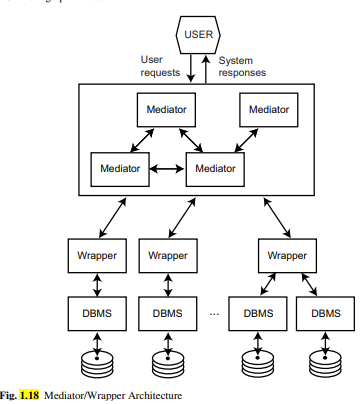
\includegraphics[width=0.8\linewidth]{image/3/1.18}

Kiến trúc trình trung gian / trình bao bọc có một số ưu điểm. Đầu tiên, các thành phần chuyên biệt của kiến ​​trúc cho phép xử lý các mối quan tâm khác nhau của các loại người dùng khác nhau một cách riêng biệt. Thứ hai, người dàn xếp thường chuyên về một tập hợp cơ sở dữ liệu thành phần có liên quan với dữ liệu “tương tự” và do đó xuất các lược đồ và ngữ nghĩa liên quan đến một miền cụ thể. Sự chuyên môn hóa của các thành phần dẫn đến một hệ thống phân tán linh hoạt và có thể mở rộng. Đặc biệt, nó cho phép tích hợp liền mạch các dữ liệu khác nhau được lưu trữ trong các thành phần rất khác nhau, từ các DBMS quan hệ chính thức đến các tệp đơn giản.

Giả sử kiến ​​trúc trình trung gian / trình bao bọc, bây giờ chúng ta có thể thảo luận về các lớp khác nhau liên quan đến quá trình xử lý truy vấn trong hệ thống cơ sở dữ liệu đa phân tán như thể hiện trong Hình 9.1.Ở đây, chúng ta giả sử đầu vào là một truy vấn về các quan hệ toàn cục được thể hiện trong phép tính quan hệ. Truy vấn này được đặt ra trên quan hệ toàn cục (phân tán), có nghĩa là phân phối dữ liệu và tính không đồng nhất bị ẩn. Ba lớp chính liên quan đến xử lý truy vấn đa cơ sở dữ liệu. Việc phân lớp này tương tự như quá trình xử lý truy vấn trong các DBMS phân tán đồng nhất (xem Hình 6.3). Tuy nhiên, vì không có phân mảnh nên không cần lớp bản địa hóa dữ liệu.

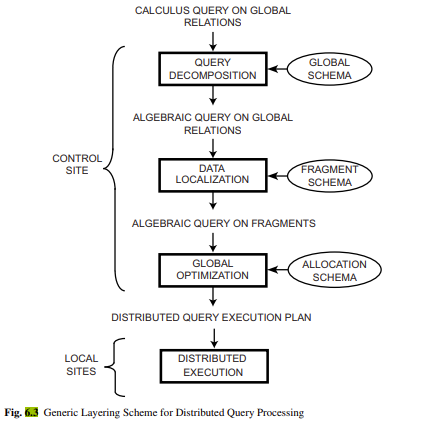
\includegraphics[width=0.8\linewidth]{image/3/6.3}

Hai lớp đầu tiên ánh xạ truy vấn đầu vào thành một kế hoạch thực thi truy vấn phân tán được tối ưu hóa (QEP). Chúng thực hiện các chức năng viết lại truy vấn, tối ưu hóa truy vấn
và một số thực thi truy vấn. Hai lớp đầu tiên được thực hiện bởi mediator và
sử dụng siêu thông tin được lưu trữ trong thư mục toàn cầu (lược đồ toàn cầu, phân bổ và
lược đồ khả năng). Viết lại truy vấn biến truy vấn đầu vào thành truy vấn trên cục bộ
quan hệ, sử dụng lược đồ toàn cục. Nhớ lại từ Chương 2 (Database Integration) rằng có hai cách tiếp cận chính để tích hợp cơ sở dữ liệu: toàn cục dưới dạng xem (GA - global as view) và cục bộ dưới dạng xem (LAV- local as view).
Do đó, lược đồ toàn cục cung cấp các định nghĩa chế độ xem (tức là, các ánh xạ giữa
quan hệ toàn cầu và quan hệ cục bộ được lưu trữ trong cơ sở dữ liệu thành phần) và
truy vấn được viết lại bằng cách sử dụng các khung nhìn.

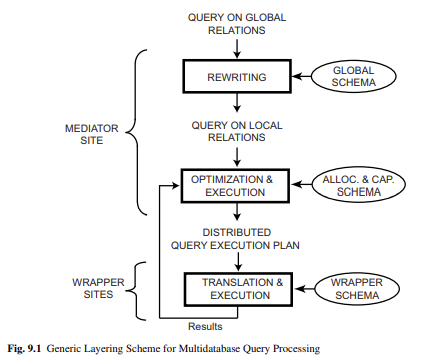
\includegraphics[width=0.8\linewidth]{image/3/9.1}

Việc viết lại có thể được thực hiện ở cấp độ giải tích quan hệ hoặc đại số. Trong chương này,
chúng ta sẽ sử dụng một dạng tổng quát của phép tính quan hệ được gọi là Datalog [Ullman, 1988]
rất thích hợp cho việc viết lại như vậy. Như vậy, có thêm một bước tính toán
sang phép dịch đại số tương tự như bước phân rã trong đồng nhất
các DBMS phân tán.

Lớp thứ hai thực hiện tối ưu hóa truy vấn và (một số) thực thi bằng cách xem xét việc phân bổ các quan hệ cục bộ và các khả năng xử lý truy vấn khác nhau
của các DBMS thành phần được xuất bởi trình bao bọc. Sự phân bổ và khả năng
lược đồ được sử dụng bởi lớp này cũng có thể chứa thông tin chi phí không đồng nhất. Các
phân phối QEP do nhóm lớp này tạo ra trong các truy vấn con các hoạt động
có thể được thực hiện bởi các DBMS thành phần và trình bao bọc. Tương tự như các DBMS được phân bổ, tối ưu hóa truy vấn có thể là tĩnh hoặc động. Tuy nhiên, việc thiếu
tính đồng nhất trong hệ thống đa cơ sở dữ liệu (ví dụ: một số DBMS thành phần có thể có
sự chậm trễ kéo dài bất ngờ trong việc trả lời) giúp tối ưu hóa truy vấn động hơn
phê bình. Trong trường hợp tối ưu hóa động, có thể có các lệnh gọi tiếp theo
lớp sau khi thực hiện bởi lớp tiếp theo. Điều này được minh họa bằng mũi tên hiển thị kết quả
đến từ lớp tiếp theo. Cuối cùng, lớp này tích hợp các kết quả đến từ các trình bao bọc khác nhau để cung cấp câu trả lời thống nhất cho truy vấn của người dùng. Điều này đòi hỏi
khả năng thực hiện một số hoạt động trên dữ liệu đến từ trình bao bọc. Kể từ khi
trình bao bọc có thể cung cấp khả năng thực thi rất hạn chế, ví dụ: trong trường hợp rất
các DBMS thành phần đơn giản, mediator phải cung cấp đầy đủ các khả năng thực thi
để hỗ trợ giao diện mediator.

Lớp thứ ba thực hiện dịch và thực thi truy vấn bằng cách sử dụng các trình bao bọc. sau đó
nó trả về kết quả cho người dàn xếp có thể thực hiện tích hợp kết quả từ
trình bao bọc và thực hiện tiếp theo. Mỗi trình bao bọc duy trì một lược đồ trình bao bọc
bao gồm lược đồ xuất cục bộ (xem Chương 4) và ánh xạ thông tin tới
tạo điều kiện thuận lợi cho việc dịch truy vấn con đầu vào (một tập hợp con của QEP) được thể hiện trong
ngôn ngữ chung thành ngôn ngữ của DBMS thành phần. Sau khi truy vấn con là
được dịch, nó được thực thi bởi DBMS thành phần và kết quả cục bộ được dịch
trở lại định dạng chung.

Lược đồ trình bao bọc chứa thông tin mô tả cách thực hiện các ánh xạ từ / đến các lược đồ cục bộ và lược đồ toàn cục. Nó cho phép chuyển đổi
giữa các thành phần của cơ sở dữ liệu theo những cách khác nhau. Ví dụ: nếu toàn cầu
giản đồ biểu thị nhiệt độ theo độ F, nhưng một cơ sở dữ liệu tham gia
sử dụng độ C, giản đồ trình bao bọc phải chứa công thức chuyển đổi thành
cung cấp bản trình bày thích hợp cho người dùng toàn cầu và cơ sở dữ liệu cục bộ. Nếu phiên bản lừa đảo có nhiều loại và các công thức đơn giản không thể thực hiện việc dịch, hãy hoàn thành
bảng ánh xạ có thể được sử dụng trong lược đồ trình bao bọc.

\subsection{Query Rewriting Using Views}
Viết lại câu truy vấn là việc định dạng lại câu truy vấn từ câu truy vấn được thể hiện trên quan hệ toàn cục(global) thành quan hệ cục bộ(local). Nó được sử dụng lược đồ toàn cục(global schema), trong đó mô tả về mặt quan điẻm sự tương ứng giữa các mối quan hệ toàn cục và quan hệ cục bộ. Do đó câu truy vấn phải được viết lại bằng cách sử dụng views. Các kỹ thuật viết lại câu truy vấn khác nhau phụ thuộc vào cách tiếp cận cơ sở dữ liệu tích hợp mà được sử dụng, tức là global-as-view (GAV) hoặc local-as-view (LAV). Phần lớn công việc viết lại câu truy vấn sử dụng views được thực hiện bằng Datalog, là một ngôn ngữ cơ sở dữ liệu dựa trên logic.Trong phần Query Rewriting Using Views này nhóm chúng em sẽ giới thiệu thuật ngữ Datalog. Sau đó sẽ mô tả kỹ thuật và thuật toán chính để viết lại truy vấn trong các cách tiếp cận GAV và LAV.
\subsubsection{Datalog Terminology}
Datalog có thể được xem như phiên bản DRC (domain relational calculus). Đầu tiên chúng ta định nghĩa conjunctive queries, thứ cơ bản cho các truy vấn phức tạp hơn. Conjunctive query trong Datalog được thể hiện như một quy tắc của form:

\[Q(T): -  R_1(T_1),...,R_n(T_n)\]
\\
Nguyên tử  $Q(T)$ là head của câu truy vấn và là biểu thị của quan hệ kết quả $R_1(T_1),...,R_n(T_n)$ là các mục tiêu phụ trong thân của câu truy vấn và là biểu thị của các quan hệ trong cơ sở dữ liệu. $Q$ và $R_1,...,R_n$ là tên vị ngữ tương ứng cho tên của quan hệ. $T,T_1,...,T_n$ tham chiếu đến bộ giá trị quan hệ và chứa các biến hoặc tham số. Các biến là tương tự như biến miền (domain variables) trong phép tính quan hệ miền (domain relational calculus). Do đó, việc sử dụng cùng một tên biến trong nhiều vị từ thể hiện các vị từ tương đương. Các hằng số tương ứng với vị từ bằng nhau. Các so sánh phức tạp hơn phải được thể hiện như các subgoal khác. Chúng ta chỉ xem xét các câu truy vấn an toàn, là các câu truy vấn mà biến xuất hiện trong head cũng phải xuất hiện trong body. Các truy vấn không hợp lệ cũng được thể hiện trong Datalog sử dụng cách kết hợp, dùng nhiều câu truy vấn liên hợp với cùng một vị từ head.
\subsubsection{Rewriting in GAV}
Trong hướng tiếp cận GAV, lược đồ toàn cục được thể hiện về mặt nguồn dữ liệu và quan hệ toàn cục được định nghĩa như một view về các quan hệ cục bộ. Điều này tương tự như lược đồ toàn cục định nghĩa trong cơ sở dữ liệu phân tán dược kết hợp chặt chẽ. Cụ thể quan hệ cục bộ có thể tương ứng cho fragments.Tuy nhiên vì cơ sở dữ liệu cục bộ tồn tại trước và là autonomous nên có thể xảy ra chuyện một tuple trong quan hệ toàn cục không tồn tại trong quan hệ cục bộ hoặc tuple trong quan hệ toàn cục xuất hiện ở quan hệ cục bộ khác. Vì thế tính chất đầy đủ và rời rạc của các mảnh có thể không dược đảm bảo. Việc thiếu tính đầy đủ có thể dẫn tới các câu trả lời không đầy đủ cho các truy vấn. Sự thiếu tính rời rạc có thể gây ra kết quả trùng lặp mà vẫn có thể là thông tin hữu ích và không cần loại bỏ.


Viết lại một truy vấn được thể hiện trên lược đồ toàn cục thành một truy vấn tương đương trên các quan hệ cục bộ là tương đối đơn giản. Kỹ thuật viết lại bằng cách sử dụng các khung nhìn được gọi là unfolding và nó thay thế mỗi quan hệ toàn cục được gọi trong truy vấn bằng khung nhìn tương ứng của nó. Điều này được thực hiện bằng cách áp dụng các quy tắc định nghĩa dạng view cho truy vấn và tạo ra một tổ hợp các truy vấn liên hợp, một truy vấn cho mỗi ứng dụng quy tắc. Vì một mối quan hệ toàn cục có thể được xác định bởi một số quy tắc, việc mở ra có thể tạo ra các truy vấn thừa cần được loại bỏ.

Mặc dù kỹ thuật cơ bản là đơn giản, việc viết lại trong GAV trở nên khó khăn khi cơ sở dữ liệu cục bộ có các mẫu truy cập hạn chế. Đây là trường hợp của các cơ sở dữ liệu được truy cập qua web nơi các quan hệ chỉ có thể được truy cập bằng cách sử dụng các mẫu ràng buộc nhất định cho các thuộc tính của chúng. Trong trường hợp này, chỉ cần thay thế các quan hệ toàn cục bằng các khung nhìn của chúng là không đủ và việc viết lại truy vấn yêu cầu sử dụng các truy vấn Datalog đệ quy.
\subsubsection{Rewriting in LAV}
Trong hướng tiếp cận LAV, lược đồ toàn cục được thể hiện là không phụ thuộc vào cơ sở dữ liệu cục bộ và mỗi quan hệ cục bộ được định nghĩa như một view về các quan hệ toàn cục. Việc này cho phép sự linh hoạt trong việc xác định các mối quan hệ cục bộ.


Việc viết lại một truy vấn được thể hiện trên lược đồ toàn cục thành một truy vấn tương đương trên các view mô tả các mối quan hệ cục bộ là khó khăn vì ba lý do. Đầu tiên, không giống như trong cách tiếp cận GAV, không có sự tương ứng trực tiếp giữa các thuật ngữ được sử dụng trong lược đồ toàn cục và các thuật ngữ được sử dụng trong các khung nhìn. Việc tìm kiếm các tương ứng yêu cầu so sánh với mỗi chế độ view.
Thứ hai, có thể có nhiều views hơn quan hệ toàn cục, do đó làm cho việc so sánh views mất nhiều thời gian. Thứ ba, các định nghĩa dạng view có thể chứa các vị từ phức tạp để phản ánh nội dung cụ thể của các quan hệ cục bộ. Do đó, không phải lúc nào cũng có thể tìm được cách viết lại tương đương của truy vấn. Trong trường hợp này, cách tốt nhất có thể làm là tìm một truy vấn chứa tối đa, tức là một truy vấn tạo ra tập con tối đa của câu trả lời.


Việc viết lại các truy vấn bằng cách sử dụng các khung nhìn đã nhận được nhiều sự quan tâm vì tính phù hợp của nó đối với các bài toán tích hợp dữ liệu vật lý và logic. Trong bối cảnh tích hợp vật lý (tức là lưu trữ dữ liệu), việc sử dụng các materialized views có thể hiệu quả hơn nhiều so với việc truy cập các quan hệ cơ sở. Tuy nhiên, vấn đề của việc tìm cách viết lại bằng cách sử dụng các views là NP-đầy đủ về số  views và số mục tiêu con trong truy vấn. Do đó, các thuật toán để viết lại một truy vấn sử dụng các khung nhìn về cơ bản cố gắng giảm số lần viết lại cần được xem xét.


Ba thuật toán chính đã được đề xuất cho mục đích này: thụât toán bucket, thuật toán inverse rule, thuật toán MinCon. Thuật toán bucket và thuật toán inverse rule có những hạn chế tương tự nhau và được giải quyết bằng thuật toán MinCon.
\subsection{Query Optimization and Execution}
Ba vấn đề chính của tối ưu hóa truy vấn trong hệ thống đa cơ sở dữ liệu là lập mô hình chi phí không đồng nhất, tối ưu hóa truy vấn không đồng nhất (để đối phó với các khả năng khác nhau của các DBMS thành phần) và xử lý truy vấn thích ứng (để đối phó với các biến thể mạnh trong môi trường - lỗi, độ trễ không thể đoán trước, v.v. ). Trong phần này, chúng tôi mô tả các kỹ thuật cho ba vấn đề này. Chúng ta lưu ý rằng kết quả là một kế hoạch thực thi phân tán sẽ được thực thi bởi wrapper và mediator.
\subsubsection{Heterogeneous Cost Modeling}
Định nghĩa hàm chi phí toàn cầu và vấn đề liên quan của việc thu thập thông tin liên quan đến chi phí từ các DBMS thành phần, có lẽ là vấn đề được nghiên cứu nhiều nhất trong ba vấn đề. Một số giải pháp khả thi đã xuất hiện, chúng ta sẽ thảo luận dưới đây. Điều đầu tiên cần lưu ý là chúng ta chủ yếu quan tâm đến việc xác định chi phí của các cấp thấp hơn của cây thực thi truy vấn tương ứng với các phần của truy vấn được thực thi tại các DBMS thành phần. Nếu chúng ta giả định rằng tất cả quá trình xử lý cục bộ được "đẩy xuống" trong cây, thì chúng ta có thể sửa đổi kế hoạch truy vấn sao cho các lá của cây tương ứng với các truy vấn con sẽ được thực thi tại các DBMS thành phần riêng lẻ. Trong trường hợp này, chúng ta đang nói về việc xác định chi phí của các truy vấn con này được nhập vào các toán tử cấp đầu tiên (từ dưới cùng). Chi phí cho các cấp cao hơn của cây thực thi truy vấn có thể được tính toán đệ quy, dựa trên chi phí nút lá. Ba cách tiếp cận thay thế tồn tại để xác định chi phí thực hiện các truy vấn tại các DBMS thành phần:
\begin{itemize}
    \item Hướng tiếp cận Black Box: hướng tiếp cận này đối xử với DBMS thành phần như một hộp đen, chạy một số truy vấn thử nghiệm trên nó và từ đó xác định thông tin chi phí cần thiết.
    \item Hướng tiếp cận Customized: hướng tiếp cận này sử dụng kiến thức trước đó về các DBMS thành phần, cũng như các đặc điểm bên ngoài của chúng để xác định một cách chủ quan thông tin chi phí
    \item Hướng tiếp cận Dynamic: Cách tiếp cận này giám sát hành vi theo thời gian chạy của các DBMS thành phần và thu thập động thông tin chi phí
\end{itemize}
\subsubsubsection{Black box approach}

Trong phương pháp tiếp cận hộp đen,
các hàm chi phí được thể hiện một cách logic (ví dụ: tổng chi phí CPU và I/O, tính chọn lọc
các yếu tố), thay vì dựa trên các đặc điểm vật lý (ví dụ, các bản chất của mối quan hệ,
số trang, số lượng các giá trị riêng biệt cho mỗi cột). Do đó, các hàm chi phí
đối với các DBMS thành phần được biểu thị bằng:
\\
\textit{Chi phí = chi phí khởi tạo + chi phí  tìm bộ giá trị đủ điều kiện + chi phí xử lí bộ giá trị đã chọn }
\\
\\
Các thành phần riêng của công thức này sẽ khác nhau đối với các toán tử khác nhau. Tuy nhiên, những khác biệt này không khó để xác định tiên nghiệm. Khó khăn cơ bản là việc xác định các hệ số thuật ngữ trong các công thức này, chúng thay đổi theo các DBMS thành phần khác nhau. Cách tiếp cận được thực hiện trong dự án Pegasus là xây dựng một cơ sở dữ liệu tổng hợp (được gọi là cơ sở dữ liệu hiệu chỉnh), chạy các truy vấn đối với nó một cách riêng biệt và đo thời gian đã trôi qua để suy ra các hệ số.


Một vấn đề với cách tiếp cận này là cơ sở dữ liệu hiệu chuẩn là nhân tạo và các kết quả thu được bằng cách sử dụng nó có thể không áp dụng tốt cho các DBMS thực. Một giải pháp thay thế được đề xuất trong dự án CORDS [Zhu và Larson, 1996b], dựa trên việc chạy các truy vấn thăm dò trên các DBMS thành phần để xác định thông tin chi phí. Trên thực tế, các truy vấn thăm dò có thể được sử dụng để thu thập một số yếu tố thông tin chi phí. Ví dụ: các truy vấn thăm dò có thể được đưa ra để truy xuất dữ liệu từ các DBMS thành phần để xây dựng và cập nhật danh mục đa cơ sở dữ liệu. Các truy vấn thăm dò thống kê có thể được đưa ra, ví dụ, đếm số bộ giá trị của một quan hệ. Cuối cùng, các truy vấn thăm dò đo lường hiệu suất có thể được đưa ra để đo thời gian đã trôi qua để xác định hệ số hàm chi phí.


Các quy tắc phân loại được định nghĩa để xác định các truy vấn thực thi tương tự và do đó có thể chia sẻ cùng một công thức chi phí. Ví dụ: người ta có thể coi rằng hai truy vấn có biểu thức đại số giống nhau (tức là cùng một hình dạng cây đại số), nhưng các quan hệ toán hạng, thuộc tính hoặc hằng số khác nhau, được thực hiện theo cùng một cách nếu các thuộc tính của chúng có cùng tính chất vật lý. Một ví dụ khác là giả sử rằng thứ tự nối của một truy vấn không ảnh hưởng đến việc thực thi vì trình tối ưu hóa truy vấn cơ bản áp dụng các kỹ thuật sắp xếp lại thứ tự để chọn một thứ tự nối hiệu quả. Do đó, hai truy vấn tham gia cùng một tập hợp quan hệ thuộc cùng một lớp, bất kỳ thứ tự nào được thể hiện bởi người dùng. Các quy tắc phân loại được kết hợp để xác định các lớp truy vấn. Việc phân loại được thực hiện từ trên xuống bằng cách chia một lớp thành những lớp cụ thể hơn hoặc từ dưới lên bằng cách hợp nhất hai lớp thành một lớp lớn hơn. Trong thực tế, một phân loại hiệu quả có được bằng cách kết hợp cả hai cách tiếp cận. Hàm chi phí toàn cầu tương tự như hàm chi phí Pegasus ở chỗ nó bao gồm ba thành phần: chi phí khởi tạo, chi phí truy xuất một bộ giá trị và chi phí xử lý một bộ giá trị. Sự khác biệt là ở cách xác định các tham số của hàm này. Thay vì sử dụng cơ sở dữ liệu hiệu chỉnh, các truy vấn mẫu được thực hiện và chi phí được đo lường. Phương trình chi phí toàn cầu được coi như một phương trình hồi quy và các hệ số hồi quy được tính toán bằng cách sử dụng chi phí đo được của các truy vấn mẫu. Các hệ số hồi quy là các tham số của hàm chi phí. Cuối cùng, chất lượng của mô hình chi phí được kiểm soát thông qua các thử nghiệm thống kê (ví dụ: F-test): nếu các thử nghiệm không thành công, phân loại truy vấn sẽ được tinh chỉnh cho đến khi đủ chất lượng. Cách tiếp cận này đã được xác nhận trên nhiều DBMS khác nhau và đã được chứng minh là mang lại kết quả tốt.
\subsubsubsection{Customized Approach}
Cơ sở của cách tiếp cận này là các bộ xử lý truy vấn của các DBMS thành phần quá khác biệt để được biểu diễn bằng một mô hình chi phí duy nhất như được sử dụng trong cách tiếp cận Black Box. Nó cũng giả định rằng khả năng ước tính chính xác chi phí của các truy vấn con cục bộ sẽ cải thiện việc tối ưu hóa truy vấn toàn cầu. Phương pháp này cung cấp một framework để tích hợp mô hình chi phí của các DBMS thành phần vào trình tối ưu hóa truy vấn dàn xếp. Giải pháp là mở rộng giao diện wrapper để mediator nhận được một số thông tin chi phí cụ thể từ mỗi wrapper. Nhà phát triển wrapper miễn phí cung cấp mô hình chi phí, một phần hoặc toàn bộ. Sau đó, thách thức là tích hợp (có thể là một phần) mô tả chi phí vào trình tối ưu hóa truy vấn trình dàn xếp. Có hai các giải pháp chính:


Giải pháp đầu tiên là cung cấp một logic trong wrapper để tính toán ba ước tính chi phí: thời gian để khởi tạo quá trình truy vấn đầu tiên (reset\_cost), thời gian để nhận item tiếp theo (advance\_cost) và số lượng kết quả. Vì thế tổng chi phí truy vấn là:

\textit{Tổng chi phí truy cập= reset\_cost + (số lượng kết quả -1) * advance\_cost}

Giải pháp này có thể mở rộng để ước lượng chi phí của các lệnh gọi thủ tục của cơ sở dữ liệu. Trong trường hợp đó wrapper cung cấp một công thức chi phí là phương trình tuyến tính phụ thuộc vào tham số thủ tục.

Giải pháp thứ hai là sử dụng mô hình chi phí chung phân cấp. Hai giải pháp vừa được trình bày rất phù hợp với kiến trúc wrapper/mediator và mang lại sự cân bằng tốt giữa chi phí cung cấp thông tin chi phí cụ thể cho các DBMS thành phần đa dạng và lợi ích của việc xử lý truy vấn không đồng nhất nhanh hơn
\subsubsubsection{Dynamic Approach}
Các cách tiếp cận trên giả định rằng môi trường thực thi ổn định theo thời gian. Tuy nhiên, trong hầu hết các trường hợp, các yếu tố môi trường thực thi thường xuyên thay đổi. Ba loại yếu tố môi trường có thể được xác định dựa trên tính thay đổi của chúng. Lớp đầu tiên cho các yếu tố thường xuyên thay đổi (mỗi giây đến mỗi phút) bao gồm CPU load, thông lượng I/O và bộ nhớ khả dụng. Lớp thứ hai cho các yếu tố thay đổi chậm (hàng giờ đến hàng ngày) bao gồm các tham số cấu hình DBMS, tổ chức dữ liệu vật lý trên đĩa và lược đồ cơ sở dữ liệu.
Lớp thứ ba cho các yếu tố gần như ổn định (hàng tháng đến hàng năm) bao gồm loại DBMS, vị trí cơ sở dữ liệu và tốc độ CPU. Chúng ta tập trung vào các giải pháp đối phó với hai lớp đầu tiên.


Một cách để đối phó với các môi trường động mà có sự tranh chấp mạng, lưu trữ dữ liệu hoặc bộ nhớ khả dụng thay đổi theo thời gian là mở rộng phương pháp lấy mẫu và coi các truy vấn của người dùng là các mẫu mới. Thời gian phản hồi truy vấn được đo để điều chỉnh các tham số của mô hình chi phí tại thời gian chạy cho các truy vấn tiếp theo. Điều này giúp tránh chi phí xử lý các truy vấn mẫu theo định kỳ, nhưng vẫn yêu cầu tính toán nhiều để giải các phương trình mô hình chi phí và không đảm bảo rằng độ chính xác của mô hình chi phí được cải thiện theo thời gian. Một giải pháp tốt hơn, được gọi là định tính, xác định mức độ tranh chấp của hệ thống là tác động tổng hợp của các yếu tố thường xuyên thay đổi lên chi phí truy vấn. Mức độ tranh chấp hệ thống được chia thành nhiều loại: cao, trung bình, thấp hoặc không có hệ thống. Điều này cho phép xác định mô hình chi phí nhiều danh mục cung cấp ước tính chi phí chính xác trong khi các yếu tố động thay đổi. Mô hình chi phí được hiệu chỉnh ban đầu bằng cách sử dụng các truy vấn thăm dò. Mức độ tranh chấp của hệ thống hiện tại được tính toán theo thời gian, dựa trên các tham số hệ thống quan trọng nhất. Cách tiếp cận này giả định rằng các lần thực thi truy vấn là ngắn, vì vậy các yếu tố môi trường không đổi trong quá trình thực thi truy vấn. Tuy nhiên, giải pháp này không áp dụng cho các truy vấn chạy dài, vì các yếu tố môi trường có thể thay đổi nhanh chóng trong quá trình thực thi truy vấn.


Để quản lý trường hợp có thể dự đoán được biến thể của yếu tố môi trường (ví dụ: tải trọng của DBMS thay đổi hàng ngày là giống nhau), chi phí truy vấn được tính cho các phạm vi ngày liên tiếp. Sau đó, tổng chi phí là tổng chi phí cho mỗi phạm vi. Hơn nữa, có thể học mẫu băng thông mạng khả dụng giữa bộ xử lý truy vấn MDBMS và thành phần DBMS. Điều này cho phép điều chỉnh chi phí truy vấn tùy thuộc vào ngày thực tế.
\subsubsection{Heterogeneous Query Optimization}
Việc tối ưu hóa truy vấn của multidatabase phải giải quyết vấn đề khả năng tính toán không đồng nhất của các DBMS thành phần. Có hai cách tiếp cận chính để giải quyết vấn đề này là:
\subsubsubsection{Query-based Approach}
Trong cách tiếp cận này các wrapper hỗ trợ cùng một khả năng truy vấn, ví dụ: một tập hợp con của SQL được dịch sang khả năng truy vấn của DBMS thành phần.
\subsubsubsection{Operator-based Approach}
Trong cách tiếp cận này các wrapper đưa ra khả năng của DBMS thành phần thông qua thành phần của các toán tử quan hệ.
\subsubsection{Adaptive Query Processing}
Xử lý truy vấn đa cơ sở dữ liệu như trong báo cáo cho tới nay tuân theo nguyên tắc xử lí truy vấn truyền thống. Giả định cơ bản trình tối ưu hóa truy vấn đa cơ sở dữ liệu có đủ kiến thức về điều kiện thời gian chạy truy vấn. Đây là một giả định hợp lý cho các truy vấn đa cơ sở dữ liệu với ít nguồn dữ liệu chạy trong môi trường dược kiểm soát. Tuy nhiên giả định này không phù hợp với môi trường thay đổi với số lượng lớn nguồn dữ liệu và điều kiện thời gian chạy không thể đoán trước.Giải pháp cho vấn đề này là có những hành vi thích nghi trong thời gian truy cập truy vấn \textit{adaptive query processing}. Là một hình thức của truy cập động các truy vấn với một vòng lặp phản hồi trong môi trường thực thi truy vấn để phản ứng lại các điều kiện thay đổi không biết trước. Môi trường thực thi bao gồm mediator, wrappers và các DBMS thành phần.
\subsubsubsection{Adaptive Query Processing Process}
Adaptive query processing thêm vào câu quá trình truy vấn thông thường các hoạt động sau: giám sát, đánh giá và phản ứng. Các hoạt động này được thực hiện một cách hợp lý trong hệ thông bởi các cảm biens, thành phần đánh giá và thành phần phản ứng tương ứng với các hoạt động. Hoạt động giám sát đo lường một số thông số môi trường trong khoảng thời gian và báo cáo cho thành phần đánh giá. Sau đó phân tích các báo cáo và xem xét các ngưỡng để đi đến một kế hoạch thích ứng. Cuối cùng kế hoạch này sẽ được thông báo cho thành phần phản ứng áp dụng các phản ứng để thực hiện truy vấn.\\
\begin{itemize}
    \item \textbf{Monitoring parameters}\\
    Giám sát các thông số theo thời gian chạy truy vấn liên quan đến việc đặt các cảm biến tại các vị trí chính của QEP và xác định các cửa sổ quan sát trong suốt quá trình cảm biến thu thập thông tin. Nó cũng yêu cầu đặc tả một cơ chế giao tiếp để chuyển thông tin thu thập được đến thành phần đánh giá. Ví dụ về các đối tượng giám sát là:
    \begin{itemize}
        \item Memory size: giám sát bộ nhớ để phản ứng lại với tình trạng thiếu hoặc tăng bộ nhớ
        \item Data arrival rates: cho phép bộ xử lí thực hiện công việc hữu ích trong khi chờ nguồn dữ liệu bị chặn.
        \item Actual statistics.
        \item Operator execution cost.
        \item Network throughput
    \end{itemize}
    \item \textbf{Adaptive reactions}\\
    Các phản ứng thích ứng thay đổi hành vi truy vấn dựa trên các quyết định đưa ra bởi thành phàn đánh giá. Các phản ứng quan trọng:
    \begin{itemize}
        \item Change schedule: thay đổi thứ tự của operator trong QEP.
        \item Operator replacement: thay đổi operator vật lý bằng một cái tương đương
        \item Operator bahavior: thay đổi hành vi vật lý của operator
        \item Data repartitioning: xem xét việc phân vùng động của mội mối quan hệ thông qua nhiều nút bằng cách sử dụng song song toán tử nội bộ
        \item Plan reformulation: tính toán một QEP mới thay thế cái cũ.
    \end{itemize}

\end{itemize}
\subsubsubsection{Eddy Approach}
Eddy là một framework cho adaptive query processing. Nó được phát triển trong bối cảnh của dự án Telegraph với mục tiêu chạy các truy vấn trên khối lượng lớn dữ liệu trực tuyến với tỷ lệ đầu vào không thể đoán trước và những biến động trong môi trường đang chạy. Chi tiết cách thích ứng của Eddy với join ordering và lập lịch:
\begin{itemize}
    \item \textbf{Adaptive join ordering}\\
    Trong Eddy không có QEP cố định, thách thức là đặt thứ tự pipelined join operator động tại thời điểm chạy khi mà các bộ giá trị từ các quan hệ khác nhau được chuyển vào. Lý tưởng nhất là khi một bộ của một quan hệ tham gia vào một join đến, nó phải được gửi tới join operator để được xử lí. Tuy nhiên hầu hết thuật toán không thể xử lý một bộ giá trị đến nhanh chóng vì chúng không đối xứng giữa bên trong và bên ngoài. Do đó cần có thuật toán đối xứng trong đó vai trò của các mối quan hệ trong phép join có thể thay đổi mà không tạo ra kết quả sai.


    Sử dụng thuật toán join đối xứng, Eddy có thể đạt được thứ tự tham gia join linh hoạt bằng cách kiểm soát lịch sử và các ràng buộc liên quan đến đánh giá vị từ dựa trên cơ sở bộ giá trị. Điều này được thực hiện dựa vào các bit tiếng trình mang theo bởi mỗi bộ giá trị, tương ứng cho biết các vị từ mà bộ giá trị đã sẵn sàng để đánh giá và tập hợp vị từ đã được đánh giá. Kết hợp thuật toán đối xứng và các bit tiến trình cho phép Eddy lập lịch các vị từ theo cách thích ứng.
    \item \textbf{Adaptive scheduling}
    Cho một bộ các vị từ, Eddy phải chọn một cách thích ứng với mỗi bộ sẽ được gửi. Hai nguyên tắc chính để chọn là chi phí và tính chọn lọc. Chi phí vị từ được đo lường như một hàm của tỷ lệ tiêu thụ mỗi vị từ. Chiến lược định tuyến của Eddy là cơ chế lập lịch xổ số đơn giản. Chiến lược gán một vé cho vị từ bất cứ khi nào vị từ sau được lên lịch một bộ giá trị. Khi một bộ giá trị được xử lý xong và trả lại cho Eddy vị từ tương ứng sẽ giảm lượng vé của nó. Việc kết hợp các tiêu chí chi phí và độ chọn lọc trở nên dễ dàng. Eddy liên tục chạy xổ số giữa các
   vị từ hiện đang yêu cầu bộ giá trị, vị từ có số lượng cao sẽ thắng vé và được xếp lịch.
\end{itemize}
\subsection{Query Translation and Execution}
Việc dịch và thực thi truy vấn được thực hiện bởi các wrapper sử dụng các cơ sở dữ liệu thành phần. Một wrapper đóng gói các chi tiết của một họăc nhiều DBMS thành phần, mỗi cơ sở dữ liệu được hỗ trợ bởi cùng một DBMS (hoặc hệ thống tệp). Nó cũng xuất cho mediator các khả năng DBMS thành phần và các chức năng chi phí trong một giao diện chung. Một trong những ứng dụng thực tế chính của wrapper là cho phép một DBMS dựa trên SQL truy cập vào cơ sở dữ liệu không phải SQL.


\subsection{Conclusion}
Xử lý truy vấn trong hệ thống đa cơ sở dữ liệu phức tạp hơn đáng kể so với trong các DBMS phân tán đồng nhất và được tích hợp chặt chẽ. Ngoài việc bị phân tán, cơ sở dữ liệu thành phần có thể tự trị, có các ngôn ngữ cơ sở dữ liệu khác nhau và khả năng xử lý truy vấn và thể hiện các hành vi khác nhau. Đặc biệt, cơ sở dữ liệu thành phần có thể bao gồm từ cơ sở dữ liệu SQL chính thức đến các nguồn dữ liệu rất đơn giản.


Giả sử kiến trúc trình mediator/wrapper phổ biến, chúng tôi đã cô lập ba lớp chính mà theo đó truy vấn được viết lại liên tiếp (chịu các quan hệ cục bộ) và được tối ưu hóa bởi bộ trung gian, sau đó được dịch và thực thi bởi các trình bao bọc và các DBMS thành phần. Chúng ta cũng đã thảo luận về cách hỗ trợ các truy vấn OLAP trong cơ sở dữ liệu đa cơ sở dữ liệu, một yêu cầu quan trọng của các ứng dụng hỗ trợ quyết định. Điều này yêu cầu một lớp dịch bổ sung từ truy vấn đa chiều OLAP sang truy vấn quan hệ. Kiến trúc phân lớp để xử lý truy vấn đa cơ sở dữ liệu nói chung là đủ để nắm bắt các biến thể rất khác nhau. Điều này rất hữu ích để mô tả các kỹ thuật xử lý truy vấn khác nhau, thường được thiết kế với các mục tiêu và giả định khác nhau. Các kỹ thuật chính để xử lý truy vấn đa cơ sở dữ liệu là viết lại truy vấn bằng cách sử dụng các khung nhìn đa cơ sở dữ liệu, tối ưu hóa và thực thi truy vấn đa cơ sở dữ liệu, dịch và thực thi truy vấn.


Các kỹ thuật viết lại truy vấn bằng cách sử dụng các khung nhìn đa cơ sở dữ liệu khác nhau theo những cách chính tùy thuộc vào việc sử dụng phương pháp tích hợp GAV hay LAV. Việc viết lại truy vấn trong GAV tương tự như việc bản địa hóa dữ liệu trong hệ thống cơ sở dữ liệu phân tán đồng nhất. Nhưng các kỹ thuật dành cho LAV (và phần mở rộng của nó là GLAV) liên quan nhiều hơn và thường không thể tìm được cách viết lại tương đương cho một truy vấn, trong trường hợp đó, một truy vấn tạo ra một tập con tối đa của câu trả lời là cần thiết. Các kỹ thuật để tối ưu hóa truy vấn đa cơ sở dữ liệu bao gồm lập mô hình chi phí và tối ưu hóa truy vấn cho các cơ sở dữ liệu thành phần với các khả năng tính toán khác nhau. Các kỹ thuật này mở rộng quá trình xử lý truy vấn phân tán truyền thống bằng cách tập trung vào tính không đồng nhất. Bên cạnh tính không đồng nhất, một vấn đề quan trọng là xử lý hành vi động của các DBMS thành phần. Xử lý truy vấn thích ứng giải quyết vấn đề này bằng cách tiếp cận động, theo đó trình tối ưu hóa truy vấn giao tiếp tại thời điểm chạy với môi trường thực thi để phản ứng với các biến thể không lường trước của điều kiện thời gian chạy. Cuối cùng, chúng ta đã thảo luận về các kỹ thuật dịch các truy vấn để thực thi bởi các DBMS thành phần và để tạo và quản lý các trình bao bọc.


Mô hình dữ liệu được mediator sử dụng có thể là mô hình quan hệ, hướng đối tượng hoặc thậm chí là bán cấu trúc (dựa trên XML). Trong phần này, để đơn giản, chúng tôi đã giả định một bộ trung gian có mô hình quan hệ đủ để giải thích các kỹ thuật xử lý truy vấn đa cơ sở dữ liệu. Tuy nhiên, khi xử lý các nguồn dữ liệu trên Web, có thể ưu tiên mô hình dàn xếp phong phú hơn như hướng đối tượng hoặc bán cấu trúc (ví dụ: dựa trên XML). Điều này đòi hỏi các phần mở rộng đáng kể cho các kỹ thuật xử lý truy vấn.
\section {References}
\textit{Özsu, M. Tamer, and Patrick Valduriez.Principles of distributed database systems.Springer Science} \& \textit{Business Media, 2011.}
\end{document}